\setlength{\parindent}{0pt}

\subsection*{Data Collection and Processing}
Data on structure and bioactivity (\% Inhibition) of compounds against HCT-116 that was used in the study was extracted from the ChEMBL website \cite{ChEMBL2023}. \% Inhibition HCT-116 database was selected due to the following reasons: a) they are widely used as benchmark cell line; and b) it is highly available \cite{Cytion_HCT116}. 
A total of 12910 entries were collected. Data with missing \% Inhibition and those that fall above the 95\% quantile was removed. This left only a total of 6304 molecule which is an amenable size for the purposes of the study. In case of imbalanced sample representation, Synthetic Minority Over-sampling Technique (SMOTE) was used \cite{gomatam2024SMOTE}. This technique involves interpolation of synthetic samples for the minority class to balance the minority and majority classes \footnote{Minority Class: $<$ 0 \% Inhibition (0), Majority Class: $>$ 0 \%Inhibition (1)}.   
%To avoid statistical error and biased prediction, the data undergoes preprocessing, which entails the removal of incomplete data and outliers. The factors considered in preprocessing were the following: a) missing values of \% Inhibition; and b) the data falls above the 95\% quantile of the data set. After preprocessing, only 6304 molecules were left, and it was used as a clean data set of the study. 

%Distribution of the uncleaned data set (Figure X) were skewed to the right, suggesting that the data are not symmetrically distributed which could lead to misleading and inaccurate predictions. Therefore, the removal of outliers (\% Inhibition greater than the 95 \% quantile and missing values) are necessary, Figure X.2 shows the improvement of data distribution which is more normal compared to uncleaned data. However, this cleaned data consist of only 6304 molecules.  

%\includegraphics[scale = 0.5]{clustering_analysis_plot.png} 

\subsection*{Generation and Visualization of Morgan Profiles and Morgan Fingerprints}

The molecules were converted into Mols from their initial SMILES format to be able to generate Morgan Fingerprints (MFP) and Morgan Profiles (MP) using the Morgan Fingerprinting Algorithm (MFA). MFA works by iterating through atoms from a randomly assigned center. Unique bit values from 0-2047 are assigned to each MFPs giving it an identification (i.e., bit ID). To create MPs, a series of structural queries is performed, noting the presence (bit value of 1) or absence (bit value of 0) until a vector of 2048 bits is achieved (\autoref{fig:mpex}). The generated MPs were used as 2D-structure representations of each molecule, while the MFPs were used as representation of molecular fingerprints/molecular fragments. To check the conversion success, MPs and MFPs were reconverted back to their respective 2D-Structures and saved as png files.

\begin{figure}[htbp!] % 'h' places the figure approximately here
	\centering
	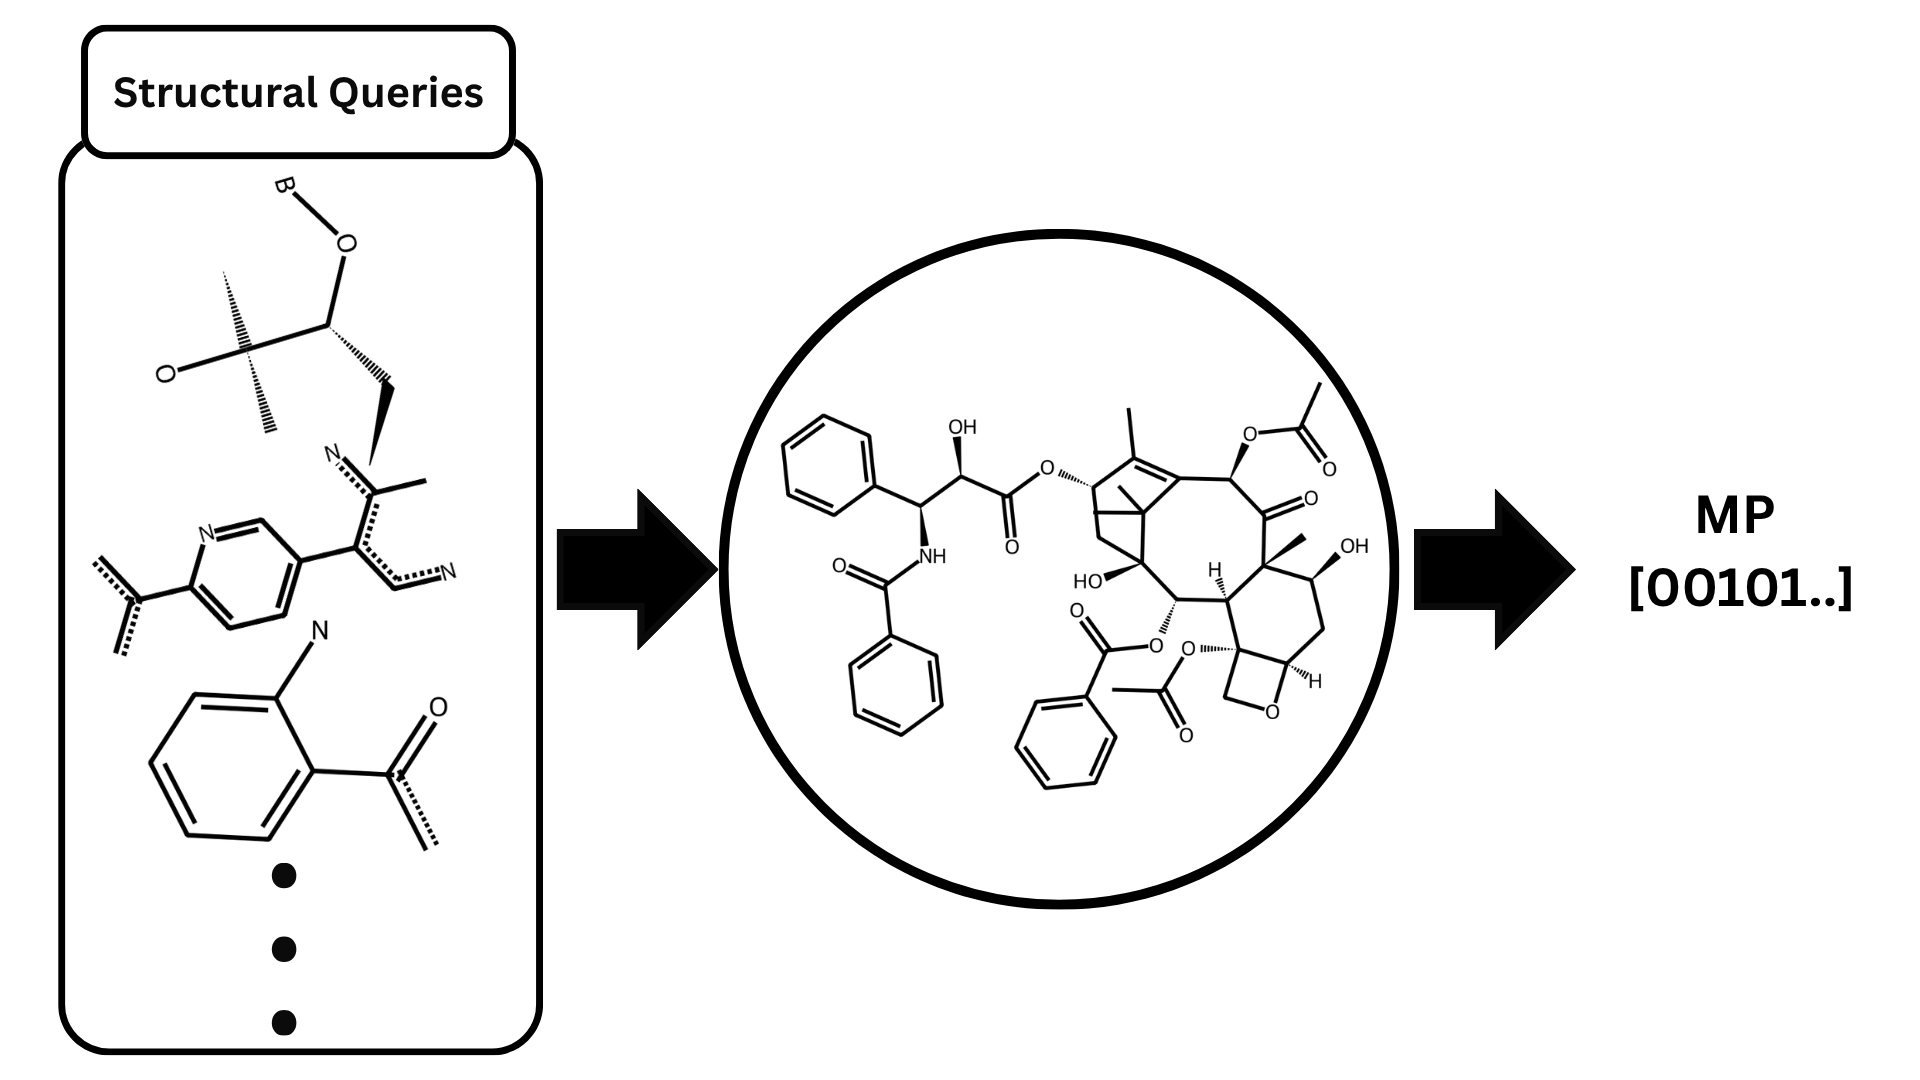
\includegraphics[scale = 0.25]{Mprofile2.png}% Replace with your image filename
	\caption{Fragmentation of target molecule to produce MFPs and MPs}
	\label{fig:mpex} % Optional: use \label for referencing
\end{figure} 

    
%after which, Morgan Fingerprinting Algorithm (MFA) parameters were set to: a) radius = 4; b) nBits = 2048; c) UseFeatures = True; and d) useChirality = True. After setting the algorithm, converted data in Mols format are feed to it which results to  generation of compounds  MP and MF. The Generated MP will become the 1-D matrix (1x2048) representation of the overall 2D-structure of each compound, which  consist of binary numbers, whereas, the MF will be the representation of molecular fingerprints/ morgan fingerprints (i.e., fragments) which were recognized as bits by the machine.

%To check if the conversion of 6304 compounds 2D-structure were successful, molecular drawing was performed through rdkit draw package. In this procedure, compounds MF's and MP's were reconverted back to its respective 2D-structures and saved as png file. In this way, the researchers were able to check the success of MP's and MF's generation via MFA. All of the data generated from these procedures were used to study the Quantitative-Structural Activity Relationship of the compounds against HCT-116.  

\subsection*{Structural Activity Relationship (SAR) of HCT-116 Compounds}
%\subsubsection{}
MFP and MP 1-D representations were used to set the ML environment. Once set, the 2D-structural data inputs can be readily perceived and interpreted by the Machine Learning Algorithm (MLA). An initial analysis of the bits was performed to categorize them before feeding to the MLA, which would allow for their assessment of significance. This is important in order to prioritize bits for subsequent feed to the MLA. When direct counting of bits was done (i.e. reflecting their absence or presence in the data set), structural queries resulted to total frequency of bits from which their ranking was based. This is the major principle in Crude Bit Counting (CBC). From the ranking, top 10 bits were used to create a CBC-ML Model, which was expected to have some capacity to predict bioactivity against HCT-116 (\autoref{fig:CBC}). On the other hand, a clustering step was also performed prior to counting, with the anticipation of shared or common features naturally emerging from the clustered molecules. This is the primary essence of Clustered Subtraction Bit Counting (CSBC).

%However, at this point there was still no way to determine which bits were significant --- there is no assessment on the weights of each bits relative to the bioactivity against HCT-116. Thus, the generated MF's were first analyzed and categorized before feeding it to the MLA. In this study, two methods were implemented to categorize and analyze the bits: CBC and CSBC.
  
%cannot identify which among the bits were significant and insignificant, hence, it lacks the ability to assess the weights of each bits relative to its bioacitivity against HCT-116. Therefore, the generated MF's were first analyzed and categorized before feeding it to the machine. In this study, two methods were implemented to categorized and analyzed the bits which are Crude Bits Counting (CBC), and Cluster-Subtraction Bits Counting (CSBC). 

\begin{figure*}[h] % 'h' places the figure approximately here
	\centering
    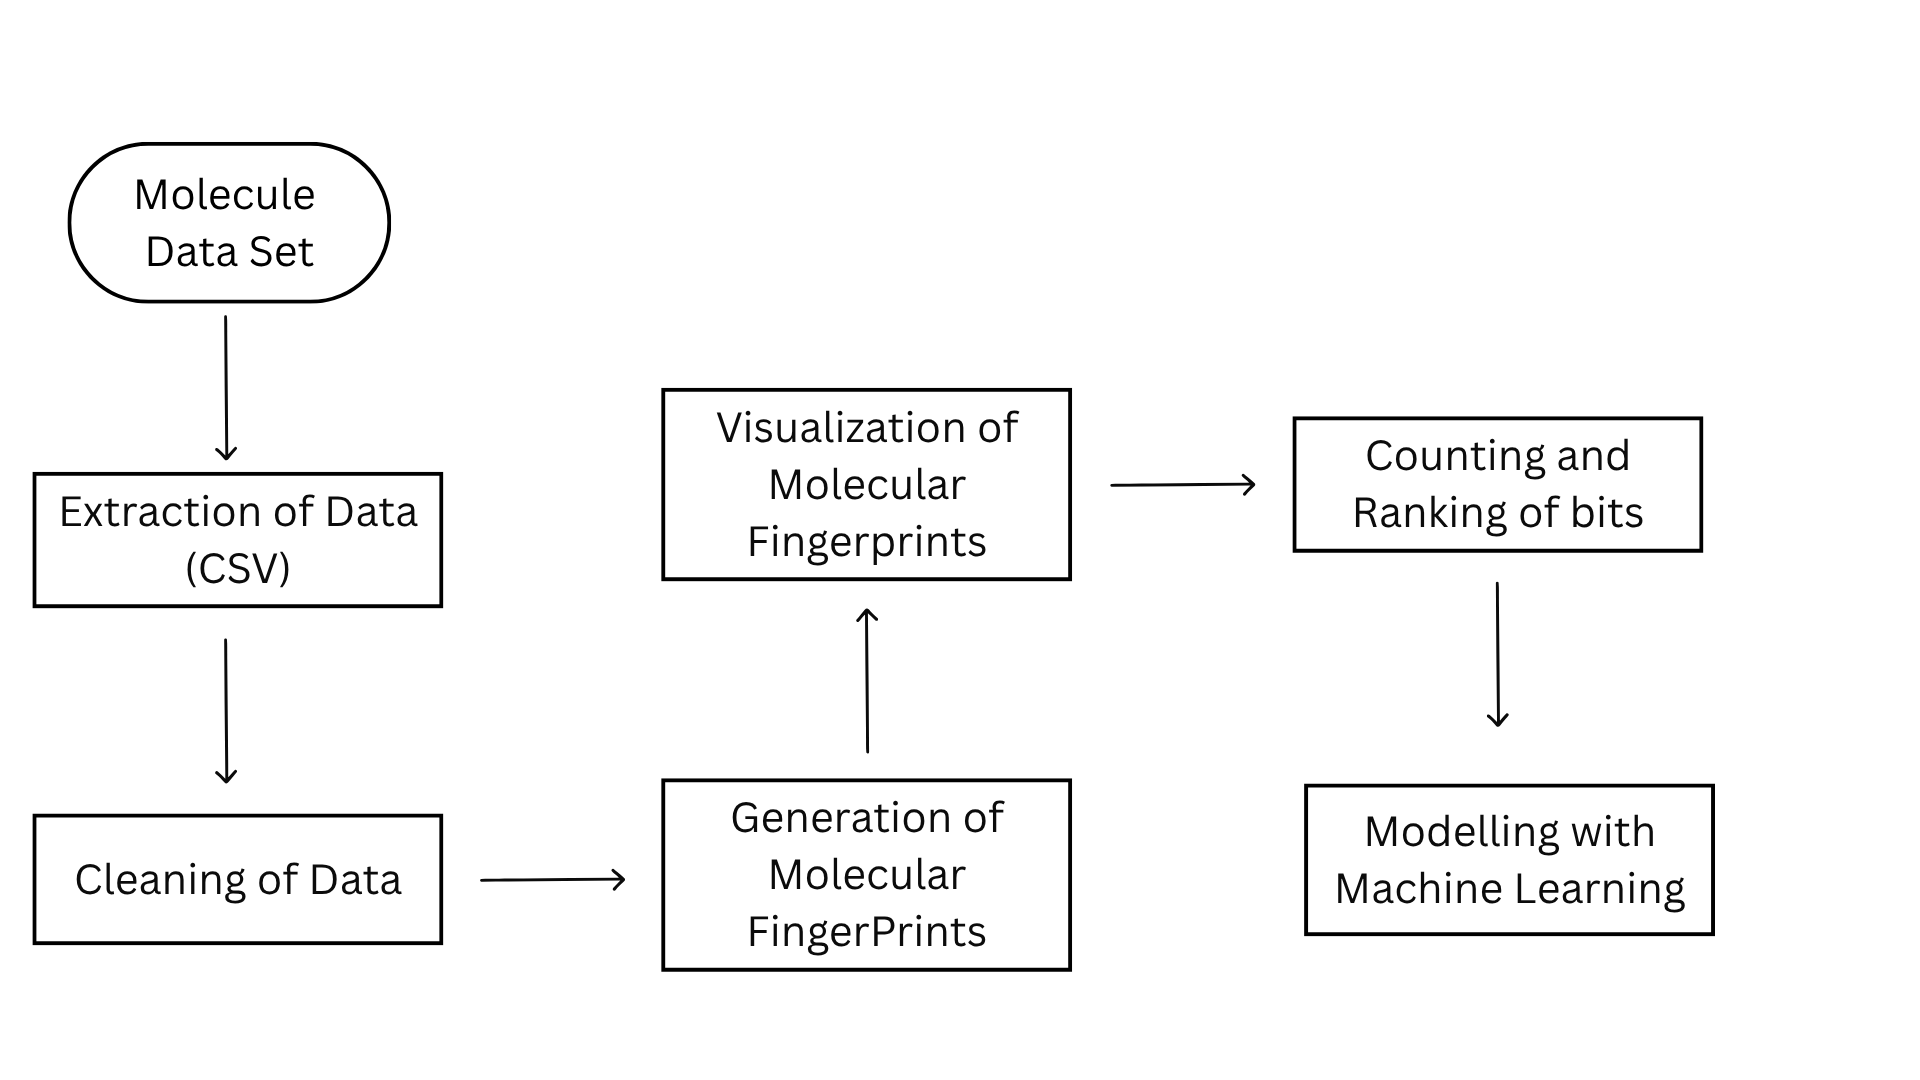
\includegraphics[scale = 0.33]{cbcv2.png}
    \vspace{-1cm} % Replace with your image filename
    \caption{Methodological framework CBC-ML}
    \label{fig:CBC} % Optional: use \label for referencing
\end{figure*}

%In CBC, after the generation and visualization of MF's and MP's, the unique bits that were produced by MFA are counted based on their presence or absence in the data set. A series of structural queries were performed to determine the total frequency of the specific bit in the given data set. After determining the total frequency of each bits, they are ranked in descending order. From the ranking, top 10 bits were used to create a CBC-ML Model, which was expected to have a capacity to perceive and classify molecules bioactivity against HCT-116 (\autoref{fig:CBC}). 

\begin{figure*}[h] % 'h' places the figure approximately here
    \centering
    \hspace{-1.05cm}
    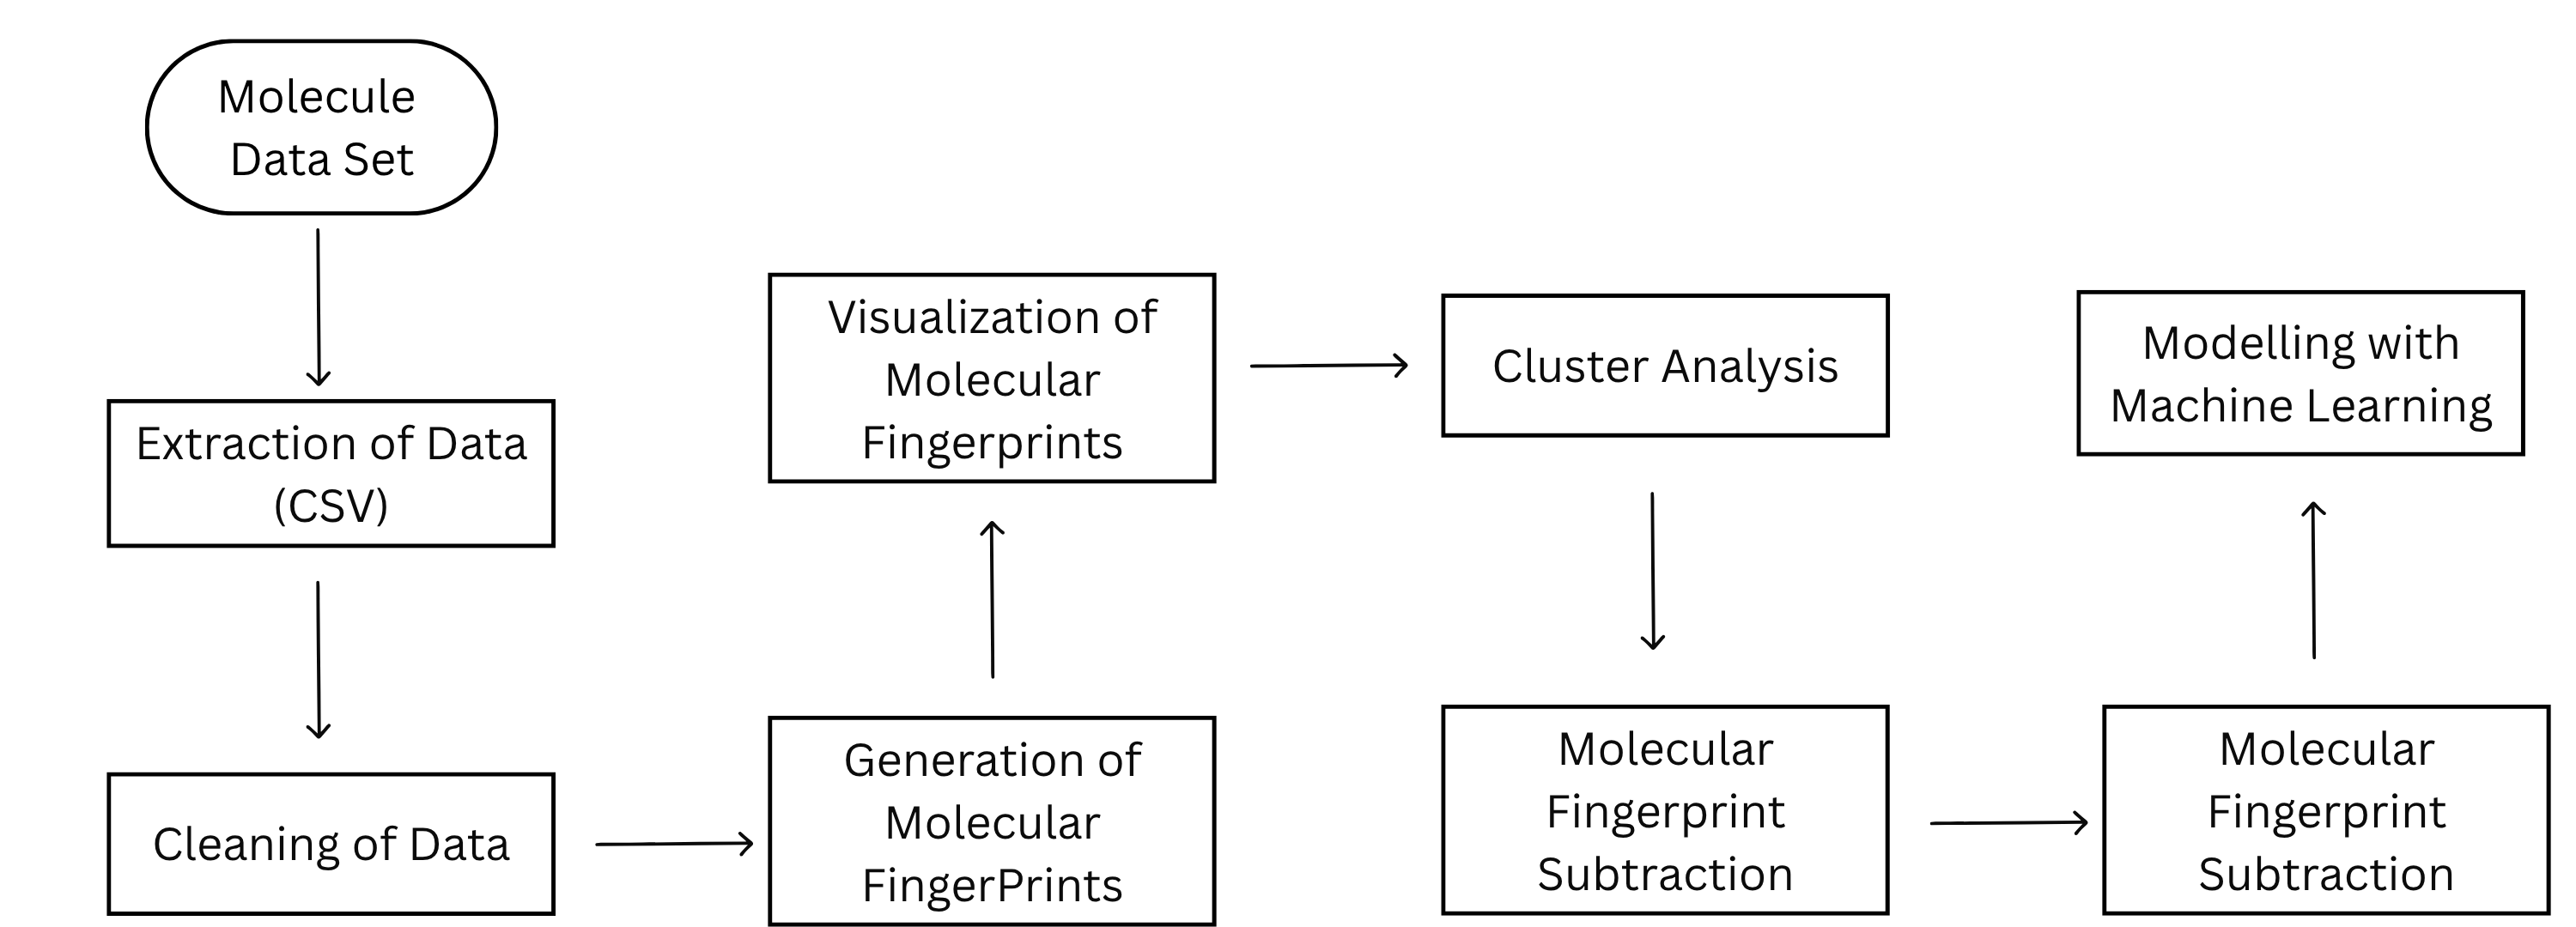
\includegraphics[scale=0.22]{csbcv2.png} % Replace with your image filename
    \caption{Methodological framework CBC-ML}
    \label{fig:CSBC} % Optional: use \label for referencing
\end{figure*}

To make sure that the optimum number of clusters was used in CSBC, Within-Cluster Sum of Squares (WCSS) (\autoref{eq:WCSS}) was computed through the elbow method. Its goal is to find the number of clusters where WCSS values converge (i.e., it does not significantly change even after increasing the number of clusters). K-Clustering was then done through the calculation of euclidean distance (\autoref{eq:euclid}) between the centroids and data points. Initially, k-seeding was performed with centroids randomly placed across the dataset. Centroid positions were then optimized based on their euclidian distances relative to a given data point (i.e., \% Inhibition). This continued until a minimum radius was achieved. The random state of the centroids in K-Clustering was set to 29. \footnote{if the random state is not set every run could have minimal variations.}

%After parameter optimization of K-Clustering it was then used to cluster clean data set of HCT-116. 

\begin{equation}
   WCSS =\sum_{i=1}^{k}\sum_{j=1}^{n_{i}}distance(x^{i}_{j},c_{i})^{2}
   \label{eq:WCSS}
\end{equation}    
where $distance(x^{i}_{j},c_{i})$ represents the distance between j-th data points $x^{i}_{j}$ in centroid $c_{i}$ and  cluster i. 

   
 \begin{equation}
    d =\sqrt{(x_{2}-x_{1})^2 +(y_{2}-y_{1})^2}
\label{eq:euclid}
\end{equation}
where d is the Euclidean distance, and $(x_{2}-x_{1}),(y_{2}-y_{1})$ are the Molecule ID and \% Inhibition respectively. 

Each cluster was then labelled under the following categories: a) High Inhibition (HI); b) Moderate Inhibition (MI); c) Low Inhibition (LI); d) Very Low Inhibition (VLI); and e) No Inhibition (NI). Since each compounds has its own MP represented by a vector, they can be added, subtracted, or multiplied. To easily categorize which among the bits were more significant than the others, MPs of compounds under VLI were subtracted from the HI, MI, LI and NI categories (\autoref{fig:subtraction}). By doing so, the bits that appear to positively contribute to the bioactivity (or positive bits, PB) the bits that negatively contribute to the bioactivity (or negative bits, NB), and the bits that appear to have no influence on bioactivity  (or non-significant bits ,NSB) were identified \footnote{PB and NB are both classified as significant bits because they positively or negatively affect the \%Inhibition of compounds against HCT-116.}. After Cluster Subtraction, the resulting vector difference underwent simplification (i.e., combination of same MPs); followed by bit frequency counting, ranking, and comparison (\autoref{fig:CSBC}). The top 16 most common bits were used for the creation of CSBC-Machine Learning Models (CSBC-ML).

\vspace{-0.55cm}
\begin{figure}[h] % 'h' places the figure approximately here
	\centering
	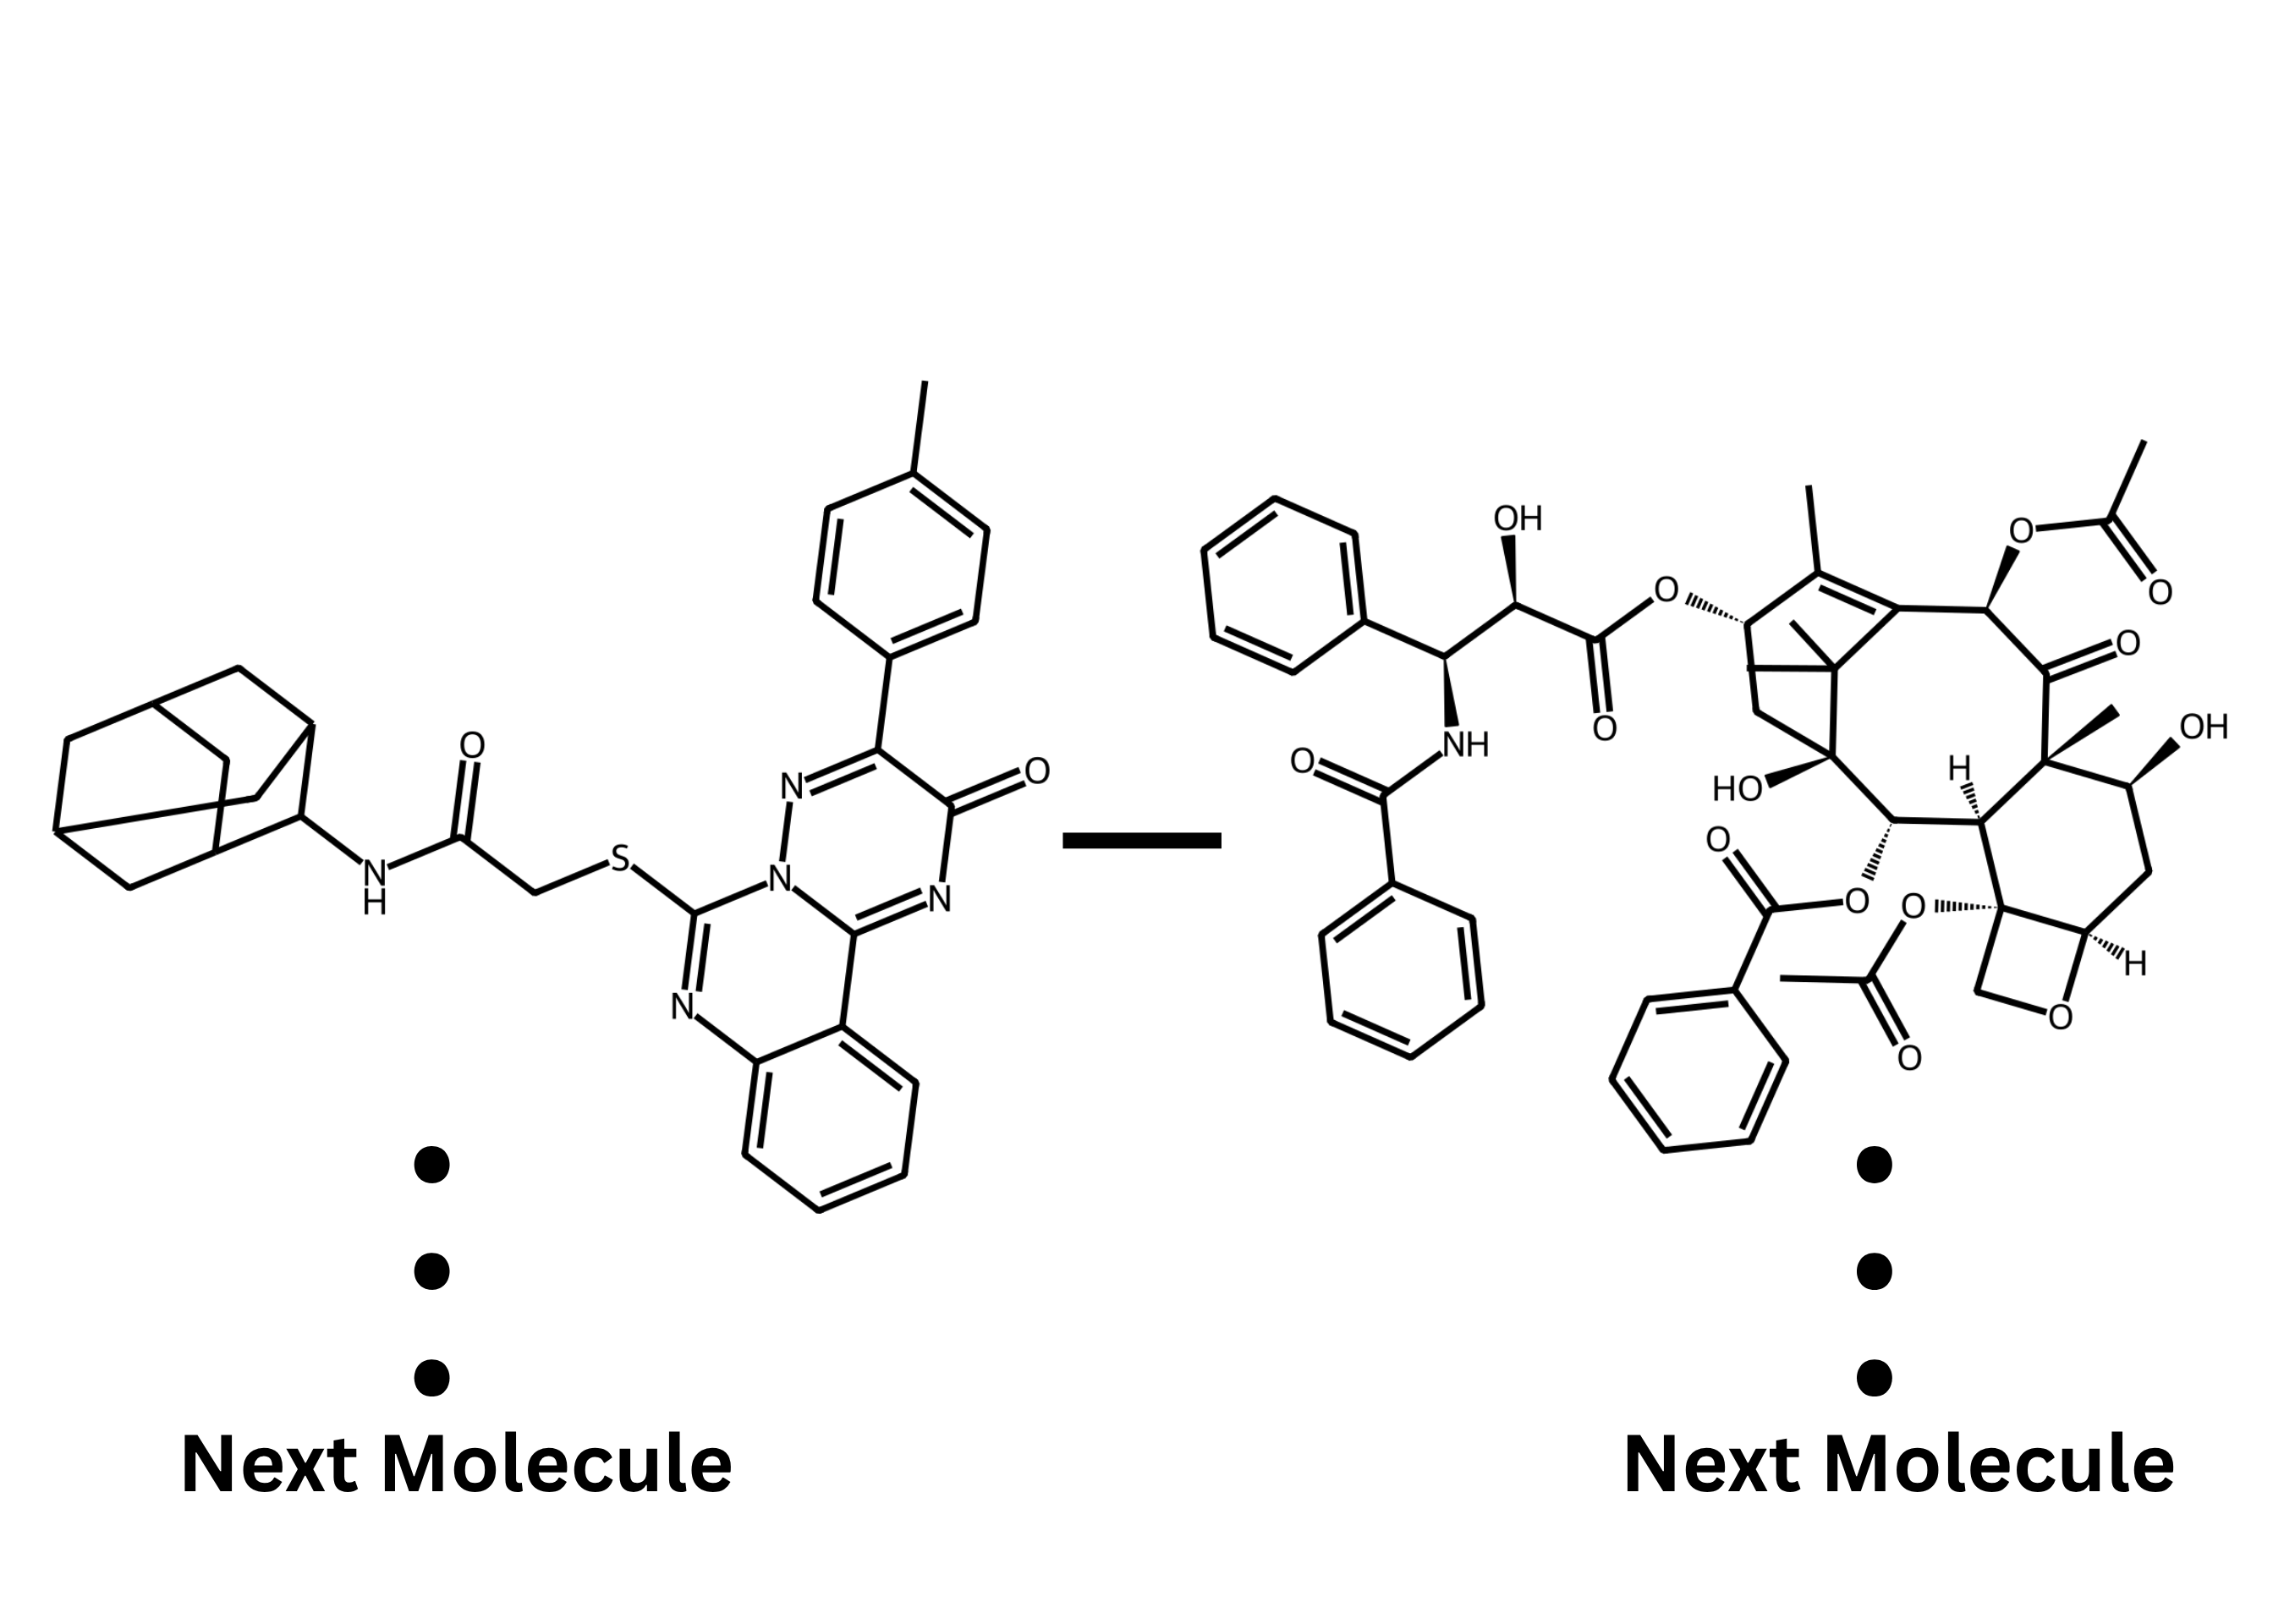
\includegraphics[width=0.57\textwidth]{mol15_minus_mol135.png} % Replace with your image filename
	\vspace{-0.5cm}
	\begin{equation*}
		\begin{bmatrix}
			1 & 0 & 1 & 0 & 1 & 1 & 1 & \ldots & 1 \\ 
			0 & 1 & 1 & 0 & 1 & 1 & 1 & \ldots & 1 \\
			\vdots & \vdots & \vdots & \vdots & \vdots & \vdots & \vdots & \ldots & \vdots \\
			0 & 1 & 1 & 0 & 1 & 1 & 1 & \ldots & 1
		\end{bmatrix}
		\text{-}
		\begin{bmatrix}
			0 & 1 & 0 & 1 & 1 & 1 & 1 & \ldots & 1 \\ 
			0 & 1 & 0 & 1 & 1 & 1 & 1 & \ldots & 1 \\
			\vdots & \vdots & \vdots & \vdots & \vdots & \vdots & \vdots & \ldots & \vdots \\
			0 & 0 & 1 & 0 & 1 & 1 & 1 & \ldots & 1
		\end{bmatrix}
		\text{=}
		\begin{bmatrix}
			1 & 0 & 1 & -1 & 0 & 0 & 0 & \ldots & 1 \\ 
			0 & 0 & 1 & -1& 0 & 0 & 0 & \ldots & 1 \\
			\vdots & \vdots & \vdots & \vdots & \vdots & \vdots & \vdots & \ldots & \vdots \\
			0 & 0 & 1 & 0 & 0 & 0 & 0 & \ldots & 1
		\end{bmatrix}
	\end{equation*}
	\caption{Structure subtraction in CSBC}
	\vspace{-0.3cm}
	\label{fig:subtraction} % Optional: use \label for referencing
\end{figure}
      
\subsection*{Quantitative Structural Activity Relationship (QSAR): CBC-ML and CSBC-ML}
The top 10, and top 16 most common structures from CBC and CSBC methods were used in the development of ML models for CBC (CBC-ML) and CSBC (CSBC-ML). These were expected to accurately perceive and classify the compounds by bioactivity against HCT-116 (active or inactive) based on their 2D-Structures. The following mathematical models were used in this study to develop the CBC-ML and CSBC-ML: a) Logistic Regression Model (Logit); b) XGBoost Model (XGB); c) Random Forest Model (RF); and d) Support Vector Machine Model (SVM) (\autoref{tab:math_models}). 

%\subsubsection*{a. CBC-ML and CSBC-ML: Mathematical Models}
\FloatBarrier % Ensures table stays below subsection

\begin{table}[h]
	\centering
	\renewcommand{\arraystretch}{1.3}
	\small
	\begin{threeparttable} % Enables footnotes
		\begin{tabular}{>{\centering\arraybackslash}p{2cm} >{\centering\arraybackslash}p{6cm} >{\centering\arraybackslash}p{6cm}}
			\hline
			\textbf{Mathematical Models} \cite{SML-formulas} & \textbf{Equations} & \textbf{Cases} \\
			\hline
			Logit \tnote{a} &  
			\begin{equation}
				y = \beta_0 + \beta_1X_1 + \beta_2X_2 + \ldots + \beta_nX_n + \epsilon
				\label{eq:logit}
			\end{equation} &  
			Performs well with linearly correlated data. \\  
			
			XGB \tnote{b} &  
			\begin{equation}
				\mathcal{L} = \sum_i l(y_i, \hat{y}_i) + \sum_k \Omega(f_k)
				\label{eq:xgboost}
			\end{equation} &  
			Can handle large datasets, imbalanced classes, and complex relationships. \\  
			
			RF \tnote{c} &  
			\begin{equation}
				f(x) = \frac{1}{M} \sum_{m=1}^M h_m(x)
				\label{eq:random}
			\end{equation} &  
			Works well with non-linear data, robust against noise and over-fitting. \\  
			
			SVM \tnote{d} &  
			\begin{equation}  
				\min \frac{1}{2} w^2 \quad \text{subject to } y_i(w \cdot x_i + b) \geq 1
				\label{eq:svm}
			\end{equation} &  
			Suitable for high-dimensional spaces, performs well for non-linear separable problems, and resistant to over-fitting. \\  
			\hline
		\end{tabular}
		\begin{tablenotes}
			\scriptsize
			\item[a] $ y $ is the target variable (\% Inhibition), $\beta_0$ is the intercept, $\beta_n$ are coefficients, and $\epsilon$ is the error term.
			\item[b] $ l(y_i, \hat{y}_i) $ is the loss function, and $ \Omega(f_k) $ is the regularization term controlling model complexity.
			\item[c] $ M $ is the total number of trees, and $ h_m(x) $ is the output from tree $ m $.
			\item[d] $ w $ is the weight vector defining the hyperplane, $ x_{i} $ are input features, $ y_{i} $ are target labels (\% Inhibition against HCT-116), and $ b $ is the bias term.
		\end{tablenotes}
	\end{threeparttable}
	\caption{Comparison of mathematical models, their underlying equations, and applicability}
	\label{tab:math_models}
\end{table}

\FloatBarrier % Prevents table from floating too far

Logit models focus (\autoref{eq:logit}) on identifying the presence and absence of a specific feature in a given query. It is based on minimizing the residual sum of squares to find the optimal parametric weights for the features. However, the Logit algorithm only works for a linearly behaved data set. For non-linear behavior, XGB, RF and SVM are best to implement due to the following reasons: a) XGB (\autoref{eq:xgboost}) involves gradient boosting iteration that gives its advantage on improving its predictions by correcting residuals during the learning process; b) RF models builds an ensemble of decision trees that are averaged to lead to a prediction; and c) SVM model finds the optimal hyperplane between the target features and its variables by adjusting its kernel functions $(K(x,x'))$(\ref{eq:svm}). The dataset used in the model development was partitioned in an 80-20 split with a random state of 29.

%\subsubsection*{a. Logit Model of CBC-ML and CSBC-ML}
%Logit Models focuses (\ref{eq:logit}) on identifying the presence and absence of a specific feature in a given query. The model is based on minimizing the residual sum of squares to find the optimal parameteric weights for the features. Fundamentally, CBC-ML and CSBC-ML were designed to accurately locate the target features (bits) in a given query (2-D structure of compounds), and to determine its specific weights. The two top bits resulting from the CBC or CSBC method were used as the features for  the CBC-ML and CSBC-ML respectively. To train and test the models, clean data set was split into train and test groups via an 80-20 partition. The models produced from this procedure are named accordingly as CBC-ML-LOG and CSBC-ML-LOG. 
%To achieved the consistency in every runs, the random state is set to 29. 

%In the training sets, the models were trained to perceived and calculate the weights of each target features, and used them to predict the compounds potency against HCT-116. Whereas, test data set were used to validate the prediction produced by the model.     

%where y is the target variable (\% Inhibition), $\beta_0$ is the intercept, ($\beta_1$, $\beta_2$ , $\ldots$, and $\beta_n$) coefficients of each features (MF/bits),($X_1$, $X_2$, $\ldots$, $X_n$) are input features (i.e., 1 & 0) and $\epsilon$ is the random error term. 

%\subsubsection*{b. XGBoost Model of CBC-ML and CSBC-ML}
%In case that the features were not linearly correlated to the target variable (\%Inhibition against HCT-116), XGBoost model were employed (\ref{eq:xgboost}). This model involves gradient boosting iteration that gives its advantage on improving its predictions by correcting residuals during the learning process. Features used in this model were the same as the Logit model and the random state was set to 29. For the development of CBC-ML-XGB and CSBC-XGB, clean data set were partitioned into 80-20 (training, testing), and the features used are the top bits from CBC and CSBC respectively.    


%where ($l(y_i, \hat{y}_i)$) is the Loss function (e.g., Mean Squared Error or Log Loss) and ($\Omega(f_k)$) is Regularization term to control model complexity. 


%\subsubsection*{c. Random Forest Model of CBC-ML and CSBC-ML}
%Random Forest Model are also effective on handling non-linear data and known to be robust against noise and overfitting (\ref{eq:random}). It builds an ensemble of decision tree that are averaged to produced a prediction. Since, the top bits could have multicollinearity characteristics, it could be detected through Random Forest Model. However, compared to Logit and XGBoost models, it is computationally intensive. For the development of CBC-ML-RF and CSBC-ML-RF, clean data set were partitioned by 80-20 with a random state of 29, and the features used were the top bits from CBC and CSBC. 


%where (M) is the total number of trees, and ($h_m(x)$) is output from tree (m). 


%\subsubsection*{d. Support Vector Machine Model of CBC-ML and CSBC-ML}
%The features used in this study were the top bits which probably have high-dimensionality, if this is the case, SVM model fits the best. SVM model aims to find the optimal hyperplane between the target features and variable. In instances of non-linearity behavior, the model kernel functions ($K(x, x')$) can be adjusted to transform the feature space (\ref{eq:svm}), making it possible for the model to handle complex and high-dimensionality data sets. However, compared to other models presented, it is memory intensive and hard to interpret. The model produced from this mathematical model were called CBC-ML-SVM and CSBC-ML-SVM, wherein the partitioned clean data set and top bits were used as the target labels and input features respectively. 


%where (w) is weight vector defining the hyperplane, ($x_{i}$) are input features, ($y_{i}$) target labels (\%Inhibition against HCT-116) and (b) is the bias term. 

\subsubsection*{Comparative Analysis of QSAR-ML Models}
Results from the four different models were assessed based on the following: a) accuracy and precision through a confusion matrix; b) model fitting of performance during training and testing; and c) overall ability of the model to distinguish between classes. The confusion matrix is a performance evaluation tool that can assess how well a model has predicted outcomes based on comparing the actual positive and negative to predicted values. It entails information about accuracy, precision, recall (sensitivity), F1 score, and specificity(\autoref{eq:accu} - \ref{eq:speci}). 

\begin{equation}
    \text{Accuracy} = \frac{\text{TP} + \text{TN}}{\text{TP} + \text{TN} + \text{FP} + \text{FN}}
    \label{eq:accu}
\end{equation}

\begin{equation}
    \text{Precision} = \frac{\text{TP}}{\text{TP} + \text{FP}}
    \label{eq:prec}
\end{equation}

\begin{equation}
   \text{Recall} = \frac{\text{TP}}{\text{TP} + \text{FN}}
   \label{eq:recall}
\end{equation}

\begin{equation}
     \text{F1 Score} = 2 \cdot \frac{\text{Precision} \cdot \text{Recall}}{\text{Precision} + \text{Recall}}
     \label{eq:f1}
\end{equation}

\begin{equation}
    \text{Specificity} = \frac{\text{TN}}{\text{TN} + \text{FP}}
    \label{eq:speci}
\end{equation}

where (TP, TN) are the true positive and true negative values, while (FP, FN) are the false positive and false negative values.

To check the performance fit of each model, the confusion matrix parameters were compared during the training and the testing stages. To evaluate the overall capability of the model to distinguish between classes (active and inactive against HCT-116), ROC, and AUC (\autoref{eq:tpr} - \ref{eq:auc}) were used. AUC helps to summarize the results from the ROC curve using the following criterion: a) AUC = 1.0 perfect classification; and b) AUC = 0.5 random guessing (no discriminatory power). A good model is expected to have the following: a) high accuracy and precision; b) a good fit (not over- or under-fitted); and c) an AUC value greater than 0.5. 

\begin{equation}
    \text{TPR} = \frac{\text{TP}}{\text{TP} + \text{FN}}
    \label{eq:tpr}
\end{equation}

\begin{equation}
    \text{FPR} = \frac{\text{FP}}{\text{FP} + \text{TN}}
    \label{eq:fpr}
\end{equation}

\begin{equation}
    \text{AUC} = \int_{0}^{1} \text{TPR}(\text{FPR}) , d(\text{FPR})
    \label{eq:auc}
\end{equation}
where TPR and FPR are the true and false positive rates.
%\subsubsection{}


